%
%===============>>  ПРОБНИК 1 <<=============
%

%BEGIN_FOLD % ====>>_____ Вариант 1 _____<<====
\begin{training}[1]
	\title{Часть 1}
	\egepreambone
	\begin{listofex}
		%1
		\item
		\begin{minipage}[t]{\bodywidth}
		Площадь треугольника \(ABC\) равна \(24\), \(DE\) --- средняя линия, параллельная стороне \(AB\). Найдите площадь треугольника \(CDE\).
			\foranswer
		\end{minipage}
		\gapwidth
		\begin{minipage}[t]{\picwidth}
				\begin{asy}
				size(5cm);
				pair A=(0,0), B=(4,0), C=(1,4);
				draw(A--B--C--cycle);
				label("$A$", A, SW);
				label("$B$", B, SE);
				label("$C$", C, N);
				pair D=(0.5, 2), E=(2.5,2);
				label("\(D\)", (A+C)/2, W);
				label("\(E\)", (B+C)/2, NE);
				draw(D--E--cycle);
				\end{asy}
		\end{minipage}
		%2
		\item
		На координатной плоскости изображены векторы \(\overrightarrow{a}\) и \(\overrightarrow{b}\). Найдите скалярное
		произведение \(\overrightarrow{a}\cdot\overrightarrow{b}\).
		\begin{center}
			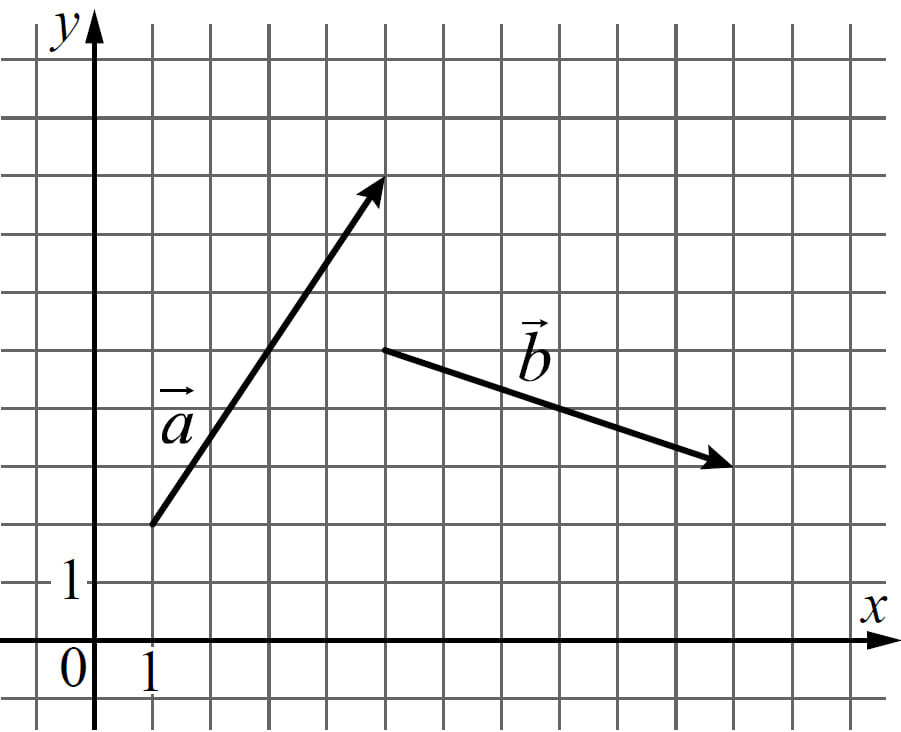
\includegraphics[align=t, width=0.4\linewidth]{\picpath/prob_23_111}
		\end{center}
		\foranswer
		%3
		\item 
		\begin{minipage}[t]{\bodywidth}
			Прямоугольный параллелепипед описан около цилиндра, радиус основания и высота которого равны \( 2 \). Найдите объём параллелепипеда.
			\foranswer
		\end{minipage}
		\gapwidth
		\begin{minipage}[t]{\picwidth}
			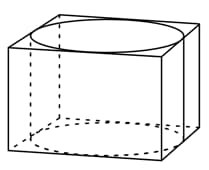
\includegraphics[align=t, width=\linewidth]{\picpath/prob_2_2}
		\end{minipage}
	\newpage
	\phantom{Часть 1}
		%4
		\item На олимпиаде по русскому языку \( 400 \) участников разместили в трёх аудиториях. В первых двух удалось разместить по \( 110 \) человек, оставшихся перевели в запасную аудиторию в другом корпусе. Найдите вероятность того, что случайно выбранный участник писал олимпиаду в запасной аудитории.
		\foranswer
		%5
		\item Симметричную игральную кость бросили \(3\) раза. Известно, что в сумме выпало
		\(6\) очков. Какова вероятность события «хотя бы раз выпало \(3\) очка»?
		\foranswer
		%6
		\item Найдите корень уравнения \( \log_9(x+6)=\log_9(4x-9) \)
		\foranswer
		%7
		\item Найдите значение выражения \( \dfrac{60n^{\tfrac{1}{18}}}{n^{\tfrac{1}{27}}\cdot n^{\tfrac{1}{54}}} \)
		\foranswer
		%8
		\item
		На рисунке изображён график функции \( y=f(x) \) и касательная к нему в точке с абсциссой \( x_0 \). Найдите значение производной функции \( f(x) \) в точке \( x_0 \).
		\begin{center}
			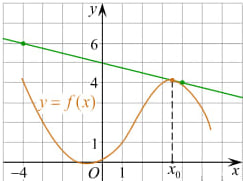
\includegraphics[align=t, width=0.4\linewidth]{\picpath/prob_2_4}
		\end{center}
		\foranswer
		%9
		\item К источнику с ЭДС \( \epsilon=55 \) В и внутренним сопротивлением \( r=0,5 \) Ом, хотят подключить нагрузку с сопротивлением \( R \) Ом. Напряжение на этой нагрузке, выражаемое в вольтах, даeтся формулой \( U=\dfrac{\epsilon R}{R+r} \).  При каком наименьшем значении сопротивления нагрузки напряжение на ней будет не менее \( 50 \) В? Ответ выразите в омах.
		\foranswer
		%10
		\item Теплоход проходит по течению реки до пункта назначения \( 247 \) км и после стоянки возвращается в пункт отправления. Найдите скорость течения, если скорость теплохода в неподвижной воде равна \( 16 \) км/ч, стоянка длится \( 7 \) часов, а в пункт отправления теплоход возвращается через \( 39 \) часов после отплытия из него. Ответ дайте в км/ч.
		\foranswer
		%11
		\item 
		На рисунке изображён график функции вида \( f(x)=ax^2+bx+c \), где числа \( a \), \( b \) и \( c \) --- целые. Найдите значение \( f(0,5) \).
		\begin{center}
			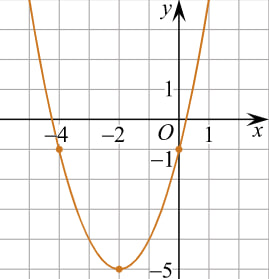
\includegraphics[align=t, width=0.4\linewidth]{\picpath/prob_2_5}
		\end{center}
		\foranswer
		%12
		\item Найдите наименьшее значение функции \( y=(x+3)^2(x+5)-1 \) на отрезке \( [-4;-1] \).
		\foranswer
		\egepreambtwo
		\title{Часть 2}
		%13
		\item a) Решите уравнение \( \cos2x+0,5=\cos^2x \). \\
		б) Найдите все корни этого уравнения, принадлежащие отрезку \( \left[ -2\pi;-\dfrac{\pi}{2} \right]  \)
		%14
		\item В основании прямой призмы \( ABCDA_1B_1C_1D_1 \) лежит квадрат \( ABCD \) со стороной \( 2 \), а высота призмы равна \( 1 \). Точка \( E \) лежит на диагонали \( BD_1 \), причём \( BE=1 \).\\
		а)  Постройте сечение призмы плоскостью \( A_1C_1E \).\\		
		б)  Найдите угол между плоскостью сечения и плоскостью \( ABC \).
		%15
		\item Решите неравенство: \( 5\cdot2^{2x+1}-21\cdot2^{x-1}\le0 \)
		%16
		\item Светлана Михайловна взяла кредит в банке на \( 4 \) года на сумму \( 4\: 420\: 000 \) рублей. Условия возврата кредита таковы: в конце каждого года банк увеличивает текущую сумму долга на \( 10\% \). Светлана Михайловна хочет выплатить весь долг двумя равными платежами --- в конце второго и четвертого годов. При этом платежи в каждом случае выплачиваются после начисления процентов. Сколько рублей составит каждый из этих платежей?
		%17
		\item В остроугольном треугольнике \( KMN \) проведены высоты \( KB \) и \( NA \).\\
		а)  Докажите, что угол \( ABK \) равен углу \( ANK \).	\\
		б)  Найдите радиус окружности, описанной около треугольника \( ABM \), если известно, что \( KN=8\sqrt{2} \) и \( \angle KMN=45\degree \).
		%18
		\item Найдите все \( a \), при каждом из которых уравнение 
		\[ \sqrt{2x+ax+2a+10}=x-1 \]
		не имеет действительных корней.
		%19
		\item Целые числа от \( 1 \) до \( n \) записаны в строчку. Под ними записаны те же числа в другом порядке. Может ли случиться так, что сумма каждого числа и записанного под ним есть точный квадрат.\\
		а)  при \( n=9 \),\\		
		б)  при \( n=11 \),\\		
		в)  при \( n=1996 \).
	\end{listofex}
\end{training}
%END_FOLD

%BEGIN_FOLD % ====>>_____ Вариант 2 _____<<====
\begin{training}[2]
	\title{Часть 1}
	\egepreambone
	\begin{listofex}
		%1
	\item
	\begin{minipage}[t]{\bodywidth}
		Отрезки \(AC\) и \(BD\) --- диаметры окружности с центром \(O\). Угол \(ACB\) равен \(61\degree\). Найдите угол \(AOD\). Ответ дайте в градусах.
		\foranswer
	\end{minipage}
	\gapwidth
	\begin{minipage}[t]{\picwidth}
		\begin{asy}
		size(6cm);
		import geometry;
		defaultpen(fontsize(10pt));
		pair A, B, C, D, O;
		A=(0,-2); C=(3.6,3.2); B=(5,0.61);
		path circ=circumcircle(A,B,C);
		D=point(circ, 0.5length(circ));
		O=circumcenter(A, B, D);
		draw(A--B--C--D);
		draw(circ);
		dot(O);
		draw(D--O--B);
		draw(A--O--C);
		label("$A$", A, SW);
		label("$B$", B, E);
		label("$C$", C, NE);
		label("$D$", D, W);
		label("$O$", O, SE);
		\end{asy}
	\end{minipage}
		%2
		\item
		Даны векторы \(\overrightarrow{a}(1;2)\), \(\overrightarrow{b} (-3;6)\), \(\overrightarrow{c} (4;-2)\). Найдите длину\\ вектора \(\overrightarrow{a}-\overrightarrow{b}+\overrightarrow{c}\).
		\foranswer
		%3
		\item
		\begin{minipage}[t]{\bodywidth}
			Через среднюю линию основания треугольной призмы проведена плоскость, параллельная боковому ребру. Площадь боковой поверхности отсеченной треугольной призмы равна \( 8 \). Найдите площадь боковой поверхности исходной призмы.
			\foranswer
		\end{minipage}
		\gapwidth
		\begin{minipage}[t]{\picwidth}
			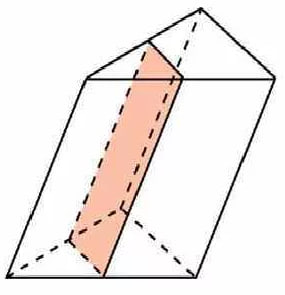
\includegraphics[align=t, width=\linewidth]{\picpath/prob_2_3}
		\end{minipage}
		%4
		\item В классе \( 16 \) учащихся, среди них два друга --- Олег и Вадим. Класс случайным образом разбивают на \( 4 \) равные группы. Найдите вероятность того, что Олег и Вадим окажутся в одной группе.
		\foranswer
		%5
		\item В городе \(48\%\) взрослого населения --- мужчины. Пенсионеры составляют \(12,6\%\) взрослого населения, причём доля пенсионеров среди женщин равна \(15\%\). Для социологического опроса выбран случайным образом мужчина, проживающий
		в этом городе. Найдите вероятность события «выбранный мужчина является пенсионером».
		\foranswer
		%6
		\item Найдите корень уравнения \(\left( \dfrac{1}{7} \right)^{x+4}=49 \).
		%\foranswer
		%\newpage
		\hphantom{Часть 1}
		%7
		\item 
		Найдите значение выражения \(6\sqrt{3}\cos^2\frac{11\pi}{12}-3\sqrt{3}\).
		\foranswer
		%8
		\item
		\begin{minipage}[t]{\bodywidth}
			На рисунке изображены график функции \(y=f(x)\) и касательная к этому графику, проведённая в точке \(x_0\). Уравнение касательной показано на рисунке. Найдите значение производной функции \(g(x)=-5f(x)-\dfrac{ 2 }{ 11 }x+\ln3\) в точке \(x_0\).
			\foranswer
		\end{minipage}
		\gapwidth
		\begin{minipage}[t]{\picwidth}
			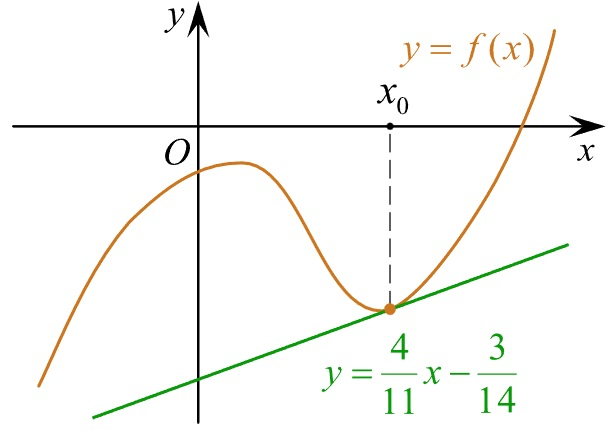
\includegraphics[align=t, width=\linewidth]{\picpath/G112M8C3-2}
		\end{minipage}
		%9
		\item В ходе распада радиоактивного изотопа его масса уменьшается по закону \( m(t)=m_0\cdot2^{-t/T} \), где \( m_0 \) --- начальная масса изотопа, \( t \) --- время, прошедшее от начального момента, \( T \) --- период полураспада. В начальный момент времени масса изотопа \( 188 \) мг. Период его полураспада составляет \( 3 \) мин. Найдите, через сколько минут масса изотопа будет равна \( 47 \) мг.
		\foranswer
		%10
		\item Имеется два сосуда. Первый содержит \( 100 \) кг, а второй --- \( 20 \) кг раствора кислоты различной концентрации. Если эти растворы смешать, то получится раствор, содержащий \( 72\% \) кислоты. Если же смешать равные массы этих растворов, то получится раствор, содержащий \( 78\% \) кислоты. Сколько килограммов кислоты содержится в первом сосуде?
		\foranswer
		\newpage
		%11
		\item 
		На рисунке изображён график функции \( f(x)=b+\log_ax \). Найдите значение \( x \), при котором \( f(x)=1 \).
		\begin{center}
			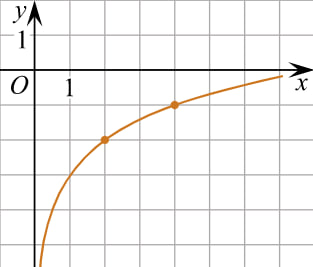
\includegraphics[align=t, width=0.4\linewidth]{\picpath/prob_2_6}
		\end{center}
		\foranswer
		%12
		\item Найдите наименьшее значение функции \( y=10\cos x+17x+3 \) на отрезке \( \left[ 0;\dfrac{3\pi}{2}\right]  \).
		\foranswer
		\egepreambtwo
		\title{Часть 2}
		%13
		\item а) Решите уравнение \( \log_2\sin2x+\log_{\frac{1}{2}}\cos x=\dfrac{1}{2} \). \\
		б) Укажите корни этого уравнения, принадлежащие отрезку \( \left[ -\dfrac{5\pi}{2};-\dfrac{\pi}{2} \right]  \).
		\newpage
		%14
		\item В основании прямой призмы \( ABCDA_1B_1C_1D_1 \) лежит квадрат \( ABCD \) со стороной \( 2 \), а высота призмы равна \( 1 \). Точка \( E \) лежит на диагонали \( BD_1 \), причём \( BE=1 \).\\
		а)  Постройте сечение призмы плоскостью \( A_1C_1E \).\\		
		б)  Найдите угол между плоскостью сечения и плоскостью \( ABC \).
		%15
		\item Решите неравенство: \( 5\cdot2^{2x+1}-21\cdot2^{x-1}\le0 \)
		%16
		\item Светлана Михайловна взяла кредит в банке на \( 4 \) года на сумму \( 4\: 420\: 000 \) рублей. Условия возврата кредита таковы: в конце каждого года банк увеличивает текущую сумму долга на \( 10\% \). Светлана Михайловна хочет выплатить весь долг двумя равными платежами --- в конце второго и четвертого годов. При этом платежи в каждом случае выплачиваются после начисления процентов. Сколько рублей составит каждый из этих платежей?
		%17
		\item В остроугольном треугольнике \( KMN \) проведены высоты \( KB \) и \( NA \).\\
		а)  Докажите, что угол \( ABK \) равен углу \( ANK \).	\\
		б)  Найдите радиус окружности, описанной около треугольника \( ABM \), если известно, что \( KN=8\sqrt{2} \) и \( \angle KMN=45\degree \).
		%18
		\item Найдите все значения \( a \), для каждого из которых уравнение \[ \log_{1-x}(a-x+2)=2 \] имеет хотя бы один корень, принадлежащий промежутку \( [-1;-1) \).
		%19
		\item Целые числа от \( 1 \) до \( n \) записаны в строчку. Под ними записаны те же числа в другом порядке. Может ли случиться так, что сумма каждого числа и записанного под ним есть точный квадрат.\\
		а)  при \( n=9 \),\\		
		б)  при \( n=11 \),\\		
		в)  при \( n=1996 \).
	\end{listofex}
\end{training}
%END_FOLD